\documentclass[11pt]{article}
\usepackage[margin=0.5in]{geometry}
\usepackage{cite}
\usepackage{graphicx}
\usepackage{appendix}
\title{Software methodologies: Image processing: A report on Non-Local Means Denoising}
\author{James Goodall}

\begin{document}
\maketitle
\section{The non-local means denoising algorithm.}

Non-local means is an algorithm for denoising images, based on the principle of replacing a pixel of an mean of all the pixels in the image weighted by how similar their surroundings are to the surroundings of the original pixel. 

As the introduction of \cite{Buades} states, the goal of image denoising methods is to recover the original image from a noisy measurement. The value of a pixel can be thought of as the sum of the original value plus a random noise element e.g.

\[P = P_0 + N\]

because of this, we can take multiple similar areas in the image we are trying to denoise, each with a different noise added to it but the same original value e.g.

\[P_1 = P_0 + N_1\]
\[P_2 = P_0 + N_2\]
\[\vdots\]
\[P_n = P_0 + N_n\]

finding the mean of $P_n$ results in the sum of $P_0$ and the average of $N$. Since $N$ can be modeled with a mean of $0$, for large values of $n$ the mean of $P_n$ tends towards $P_0$

\subsection{The Algorithm} \label{algorithm}

the algorithm is defined by \cite{Buades_2005} to be: 

\[NL(v)(i) = \sum_{j \in I}{w(i,j)v(j)}\]

with $w(i,j)$ being the similarity function, which is the square of the euclidian distance between the two areas surrounding the pixels i and j, calculated by:

\[\left\|v\left(\mathcal{N}_{i}\right)-v\left(\mathcal{N}_{j}\right)\right\|_{2, a}^{2}\]

with $\mathcal{N}_i$ refering to the pixels surrounding i

A useful property of this similarity function is that, as explained in \cite{Buades_2005} is that the Euckudean distance preserves the order of similarity between pixels, which is to say, that the similarity of $a$ to $b$ is the same as the similarity of $b$ to $a$.

\section{Implementations of the algorithm and their efficiency.}

There are two main implementations of the algorithm, pixelwise and patchwise:

\subsection{Pixelwise}

The pixelwise implemtation is as described in section \ref{algorithm}, howevere due to computational limitations, in \cite{Buades_2011}, the search windows, instead of being the entire image, is limited to a $21\times 21$ square around the pixel in question for small values of $\sigma$ and to a $35 \times 35$ square for large values.

\subsection{Patchwise}

The patchwise implementation of the algorithm is similar to the pixelwise, except that it is applied to a patch instead of a pixel, and the final value of each pixel is the mean value of all the patches it is part of.

The Patchwise implementation has an algorithmic complexity of $N^2(2f + 1)^2$ where f is the patch size.

\section{The influence of the algorithmic parameters on the output.}

\begin{figure}
    \centering
    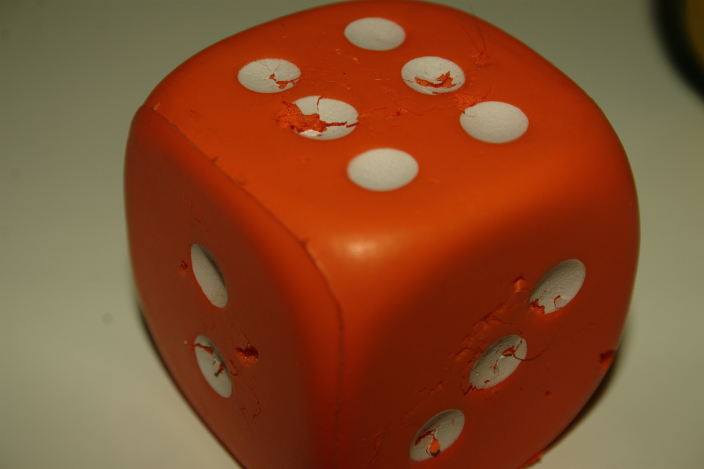
\includegraphics[width=0.2\linewidth]{Images/dice.png}
    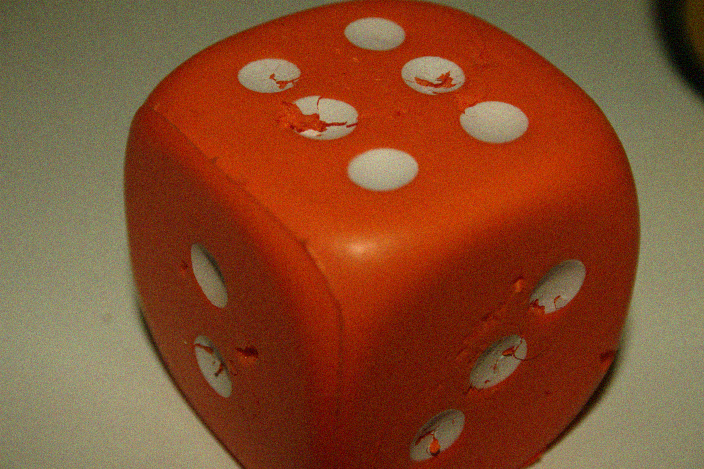
\includegraphics[width=0.2\linewidth]{Images/dice-Noise.png}
    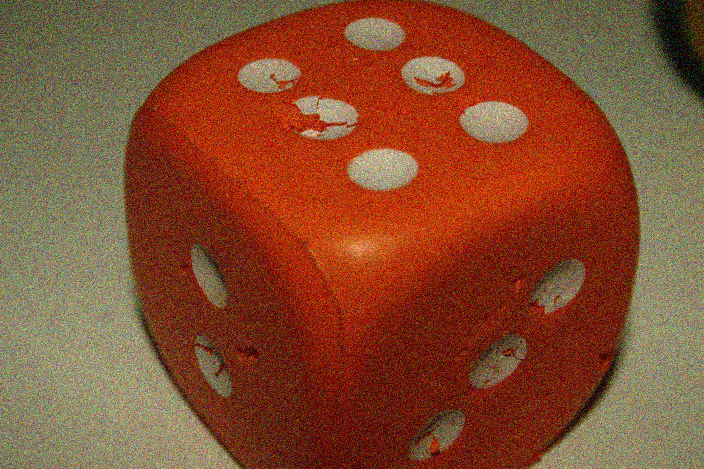
\includegraphics[width=0.2\linewidth]{Images/dice-highNoise.png}
    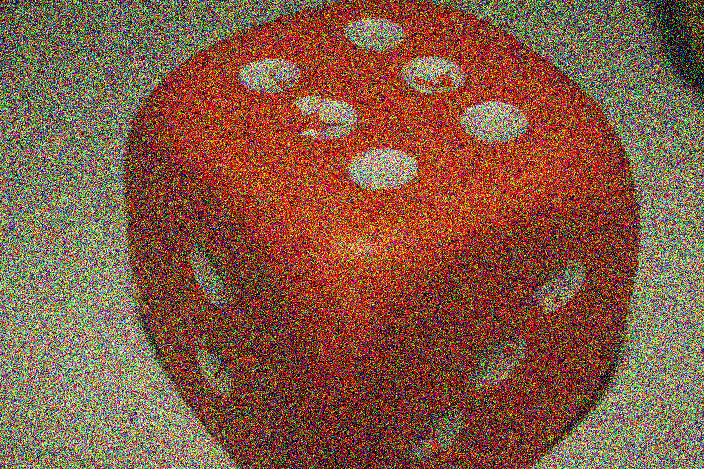
\includegraphics[width=0.2\linewidth]{Images/dice-extremeNoise.png}
    \caption{An image of a die, with progressivly more noise}
    \label{fig:diceNoiseProgression}
\end{figure}

Figure \ref{fig:diceNoiseProgression} shows the image we are going to use to demonstrate the effects of the algorithms parameters.

\subsection{h}

\begin{figure}
    \centering
    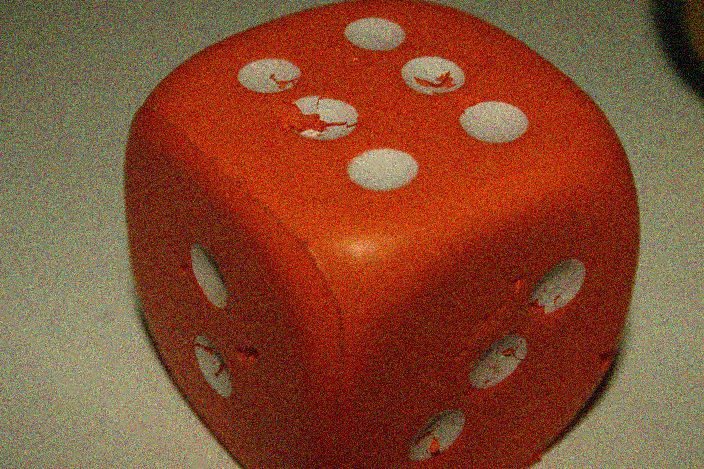
\includegraphics[width=0.2\linewidth]{Images/dice-high-5-7-35.png}
    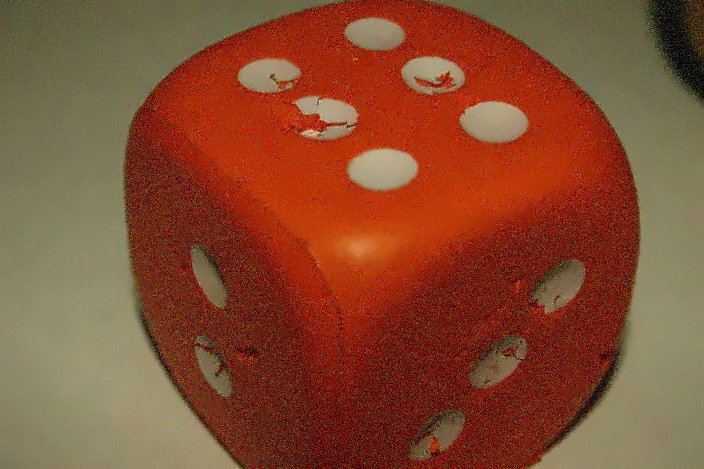
\includegraphics[width=0.2\linewidth]{Images/dice-high-10-7-35.png}
    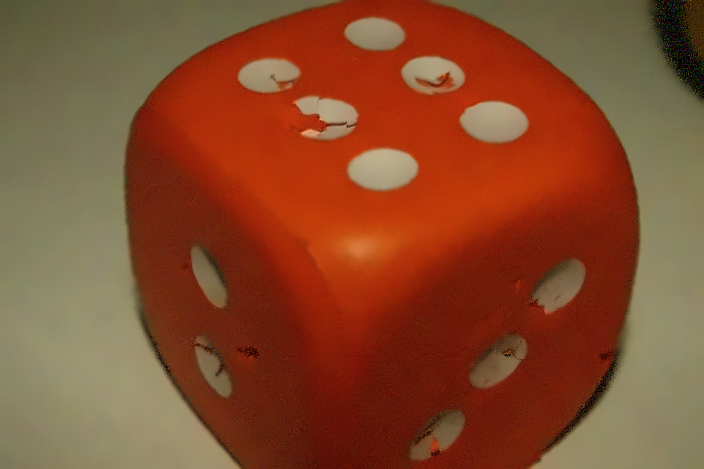
\includegraphics[width=0.2\linewidth]{Images/dice-high-15-7-35.png}
    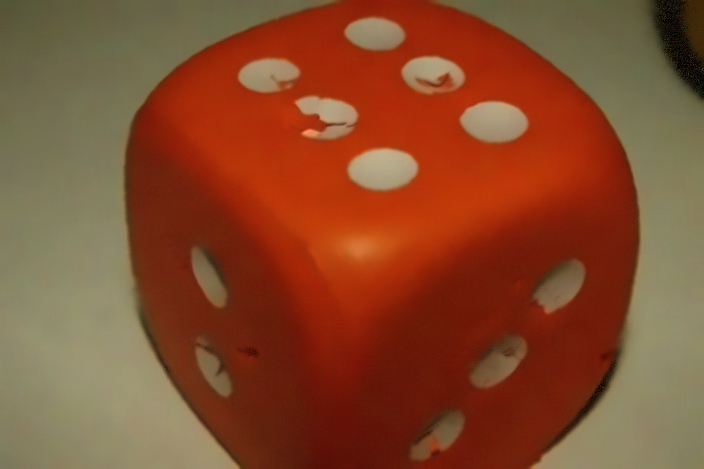
\includegraphics[width=0.2\linewidth]{Images/dice-high-20-7-35.png}
    \caption{As h increases, the amount of noise visible in the image decreases}
    \label{fig:diceHProgression}
\end{figure}

h is the strength of the denoising effect of the algorithm, as can be seen in figure \ref{fig:diceHProgression}. As h increases, the amount of noise the algorithm removes also increases. Eventually, as h increases, the image will start to lose large amounts of detail and become blury.

\subsection{Template Window Size}

The template window size is the area of the image that is searched for similar areas, as it increases, the quality of the noise reduction increases, as more areas will be searched, however, the computational load to denoise the image increases.

\subsection{Search Window Size}

The search window size is the size of the area around the target pixel which is compared. increasing this will slightly increase the quality of the denoising as it will lead to a more accurate representation of which pixels are similar to the target pixel, however, increasing it also increases the computational complexity of the algorithm.

\section{The strengths and limitations of non-local means compared to other denoising algorithms. }


Based on the work done \cite{Buades_2005}, and Figure \ref{fig:compare}, the following comparisons can be made:

\begin{figure}
    \centering
    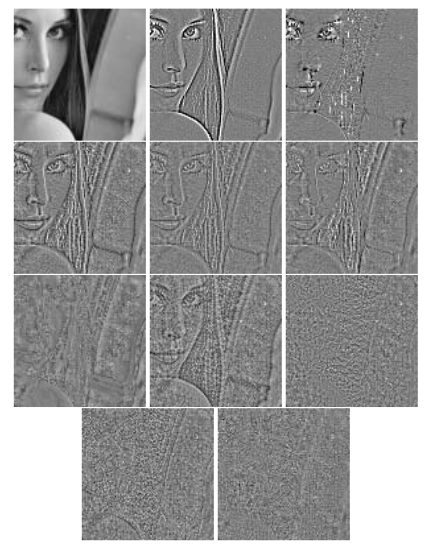
\includegraphics[width=0.5\linewidth]{Images/compare.png}
    \caption{From left to right and top to bottom, original image, Gaussian convolution, mean curvature motion, total variation, Tadmor–Nezzar–Vese iterated total variation, Osher et al. total variation, neighborhood filter, soft TIWT, hard TIWT, DCT empirical Wiener filter, and the NL-means algorithm. the closer to white noise the image is, the better the better the denoising, Image taken from \cite{Buades_2005}, Fig 15} 
    \label{fig:compare}
\end{figure}

In Figure \ref{fig:compare}, it is clear that NL-means results in an image significantly closer to white noise than many of the other algorithms, this means that over the entire image, there are no specific features that are largely changed from the original image, wheras with many of the other algorithms, there are large features, e.g. the hard edges in the photograph that are degraded/blured a large amount.

As \cite{Buades_2005} explains, the NL-means algorithm performs well on periodic images, that is, images which have a pattern or texture that repeats periodically. This is because the algorithm can find many other iterations of the area surrounding the corrupted pixel, wheras other local smoothung algorithm will just use pixels part of the same iteration of the pattern

Since NL-means, at least in its theoretical form, without any artificial limitations, compares every pixel against every other pixel, it has a computational complexity of $O(N^2)$. wheras local algorithms tend to only compare each pixel with the pixels around it and therefore are closer to linear. This means that, compared to other algorithms, NL-means theoretically runs slightly slower.

\section{Modifications and extensions of the algorithm that have been proposed in the literature.}

An extension of the algorithm that has been proposed in \cite{Tasdizen_2008} is to use principle component analysis (PCA) to significantly reduce the dimentionality of the similarity calculation.

The idea is to model the image neighbourhood as a vector (e.g. for a $7 \times 7$ neighbourhood, 49 dimensions would be used) and find a number of principle components e.g. 6. Then, when comparing the similarities between neighbourhoods, find the Euclidian distance between the values in the 6 principle components for the areas. 

Because the Euclidian distance is calculated between two only 6 dimentional vectors rather than two 49 dimentional vectors, \cite{Tasdizen_2008} finds that the computational cost of the non-local means algorithm is improved upon, and because the dimensions chosen are principle components, this can be achieved without a large loss in quality.

\section{Applications of the original algorithm and its extensions. }

A couple of interesting applications of the algorithm have been proposed. 

\subsection{A view interpolation method without explicit disparity estimation}

\cite{Dehghannasiri_2013} proposes the use of the NL-means algorithm for view interpolation. "Using NL-means, every pixel in the intermediate view is set to a weighted linear combination of the avererages of pairs of pixels in the reference views.", "The main ben-efit of this method is that it does not require explicit dispar-ity estimation.  Experimental results show that the proposedmethod outperforms other view interpolation algorithms."

\subsection{Depth estimation from a video sequence with moving and deformable objects.}

\cite{Martinello_2012} proposes the use of the NL means algorithm for depth estimation from a single video source. They propose to apply the non-local filtering to both the spacial and temporal domains with the assumption that regions with a similar texture in the same frame and neighbouring frames are likely to belong to the same surface. 

\bibliography{research}
\bibliographystyle{plain}

\end{document}
